% Style from https://stackoverflow.com/questions/1911516/how-to-make-cheat-sheets-in-latex/36768704#36768704
\documentclass[10pt,landscape,a4paper]{article}
\usepackage[utf8]{inputenc}
\usepackage[english]{babel}
\usepackage{amssymb}
\usepackage{amsmath}
\usepackage{tikz,pgf}
\usepackage{pgfplots}
\usetikzlibrary{angles,shapes,positioning,arrows,fit,calc,graphs,graphs.standard}
\usepackage{multicol}
\usepackage{wrapfig}
\usepackage[top=0mm,bottom=1mm,left=0mm,right=1mm]{geometry}
\usepackage[framemethod=tikz]{mdframed}
\usepackage{microtype}

\let\bar\overline

\DeclareMathOperator{\re}{Re}
\DeclareMathOperator{\im}{Im}
\DeclareMathOperator{\caparg}{Arg}

\newcommand{\abs}[1]{\left|#1\right|}           % absolute value
\newcommand{\Arg}[1]{\caparg #1}
\renewcommand{\bar}[1]{\mkern 1.5mu \overline{\mkern -1.5mu #1 \mkern -1.5mu} \mkern 1.5mu}

\pgfplotsset{compat=1.15}
\usepgfplotslibrary{fillbetween}
\pgfplotsset{four quads/.append style={axis x line=middle, axis y line=
middle, xlabel={$x$}, ylabel={$y$}, axis equal }}
\pgfplotsset{four quad complex/.append style={axis x line=middle, axis y line=
middle, xlabel={$\re$}, ylabel={$\im$}, axis equal }}

\definecolor{myblue}{cmyk}{1,.72,0,.38}

\def\firstcircle{(0,0) circle (1.5cm)}
\def\secondcircle{(0:2cm) circle (1.5cm)}

\colorlet{circle edge}{myblue}
\colorlet{circle area}{myblue!5}

\tikzset{filled/.style={fill=circle area, draw=circle edge, thick},
    outline/.style={draw=circle edge, thick}}

\pgfdeclarelayer{background}
\pgfsetlayers{background,main}

\everymath\expandafter{\the\everymath \color{myblue}}
\everydisplay\expandafter{\the\everydisplay \color{myblue}}

\renewcommand{\baselinestretch}{.8}
\pagestyle{empty}

\global\mdfdefinestyle{header}{%
linecolor=gray,linewidth=1pt,%
leftmargin=0mm,rightmargin=0mm,skipbelow=0mm,skipabove=0mm,
}

\newcommand{\header}{
\begin{mdframed}[style=header]
\footnotesize
\sffamily
PMATH352W18 Cheatsheet\\
by~Johnson~Ng,~page~\thepage~of~1
\end{mdframed}
}

\makeatletter
\renewcommand{\section}{\@startsection{section}{1}{0mm}%
                                {.2ex}%
                                {.2ex}%x
                                {\color{myblue}\sffamily\small\bfseries}}
\renewcommand{\subsection}{\@startsection{subsection}{1}{0mm}%
                                {.2ex}%
                                {.2ex}%x
                                {\sffamily\bfseries}}



\def\multi@column@out{%
   \ifnum\outputpenalty <-\@M
   \speci@ls \else
   \ifvoid\colbreak@box\else
     \mult@info\@ne{Re-adding forced
               break(s) for splitting}%
     \setbox\@cclv\vbox{%
        \unvbox\colbreak@box
        \penalty-\@Mv\unvbox\@cclv}%
   \fi
   \splittopskip\topskip
   \splitmaxdepth\maxdepth
   \dimen@\@colroom
   \divide\skip\footins\col@number
   \ifvoid\footins \else
      \leave@mult@footins
   \fi
   \let\ifshr@kingsaved\ifshr@king
   \ifvbox \@kludgeins
     \advance \dimen@ -\ht\@kludgeins
     \ifdim \wd\@kludgeins>\z@
        \shr@nkingtrue
     \fi
   \fi
   \process@cols\mult@gfirstbox{%
%%%%% START CHANGE
\ifnum\count@=\numexpr\mult@rightbox+2\relax
          \setbox\count@\vsplit\@cclv to \dimexpr \dimen@-1cm\relax
\setbox\count@\vbox to \dimen@{\vbox to 1cm{\header}\unvbox\count@\vss}%
\else
      \setbox\count@\vsplit\@cclv to \dimen@
\fi
%%%%% END CHANGE
            \set@keptmarks
            \setbox\count@
                 \vbox to\dimen@
                  {\unvbox\count@
                   \remove@discardable@items
                   \ifshr@nking\vfill\fi}%
           }%
   \setbox\mult@rightbox
       \vsplit\@cclv to\dimen@
   \set@keptmarks
   \setbox\mult@rightbox\vbox to\dimen@
          {\unvbox\mult@rightbox
           \remove@discardable@items
           \ifshr@nking\vfill\fi}%
   \let\ifshr@king\ifshr@kingsaved
   \ifvoid\@cclv \else
       \unvbox\@cclv
       \ifnum\outputpenalty=\@M
       \else
          \penalty\outputpenalty
       \fi
       \ifvoid\footins\else
         \PackageWarning{multicol}%
          {I moved some lines to
           the next page.\MessageBreak
           Footnotes on page
           \thepage\space might be wrong}%
       \fi
       \ifnum \c@tracingmulticols>\thr@@
                    \hrule\allowbreak \fi
   \fi
   \ifx\@empty\kept@firstmark
      \let\firstmark\kept@topmark
      \let\botmark\kept@topmark
   \else
      \let\firstmark\kept@firstmark
      \let\botmark\kept@botmark
   \fi
   \let\topmark\kept@topmark
   \mult@info\tw@
        {Use kept top mark:\MessageBreak
          \meaning\kept@topmark
         \MessageBreak
         Use kept first mark:\MessageBreak
          \meaning\kept@firstmark
        \MessageBreak
         Use kept bot mark:\MessageBreak
          \meaning\kept@botmark
        \MessageBreak
         Produce first mark:\MessageBreak
          \meaning\firstmark
        \MessageBreak
        Produce bot mark:\MessageBreak
          \meaning\botmark
         \@gobbletwo}%
   \setbox\@cclv\vbox{\unvbox\partial@page
                      \page@sofar}%
   \@makecol\@outputpage
     \global\let\kept@topmark\botmark
     \global\let\kept@firstmark\@empty
     \global\let\kept@botmark\@empty
     \mult@info\tw@
        {(Re)Init top mark:\MessageBreak
         \meaning\kept@topmark
         \@gobbletwo}%
   \global\@colroom\@colht
   \global \@mparbottom \z@
   \process@deferreds
   \@whilesw\if@fcolmade\fi{\@outputpage
      \global\@colroom\@colht
      \process@deferreds}%
   \mult@info\@ne
     {Colroom:\MessageBreak
      \the\@colht\space
              after float space removed
              = \the\@colroom \@gobble}%
    \set@mult@vsize \global
  \fi}

\makeatother
\setlength{\parindent}{0pt}

\begin{document}
\small
\begin{multicols*}{5}
\section{Complex Numbers and Their Properties}
\subsection*{Complex Plane as a Set}
$\mathbb{C} = \mathbb{R}^2 = \left\{\begin{pmatrix} x \\ y \end{pmatrix} : x, y \in \mathbb{R} \right\}$
\subsection*{Real and Imaginary Part}
$\forall z = x + iy \in \mathbb{C} \; x, y \in \mathbb{R} \\ \re(z) = x \; \im(z) = y$
\subsection*{Product}
$\forall z = a + ib, w = c + id \in \mathbb{C} \; a, b, c, d \in \mathbb{R} \\
zw = (ac - bd) + i (ad + bc)$
\subsection*{Inverse of a Complex Number}
$\forall z = a + ib \in \mathbb{C} \; a, b \in \mathbb{R} \\
\exists z^{-1} = \frac{a}{aa^2 + b^2} - i \frac{b}{a^2 + b^2} \in \mathbb{C}$
\subsection*{Conjugate}
$\forall z = a + ib \in \mathbb{C} \; a, b \in \mathbb{R} \\
\exists \bar{z} = a - ib \in \mathbb{C}$
\subsection*{Modulus}
$\forall z = x = iy \in \mathbb{C} \; x, y \in \mathbb{R} \\
\abs{z} = \sqrt{x^2 + y^2} \in \mathbb{R}$
\subsection*{Basic Inequalities}
$\forall z, w \in \mathbb{C},$
\begin{enumerate}
	\item $\abs{\re(z)} \leq \abs{z}$
	\item $\abs{\im(z)} \leq \abs{z}$
	\item $\abs{z + w} \leq \abs{z} + \abs{w}$
	\item $\abs{z + w} \geq \abs{ \; \abs{z} + \abs{w} \; }$
\end{enumerate}
\subsection*{Region of a set of Complex Numbers}
Describe $\{z \in \mathbb{C} : \abs{z - a} < \abs{z - b}\}$.
\resizebox{\columnwidth}{!}{
	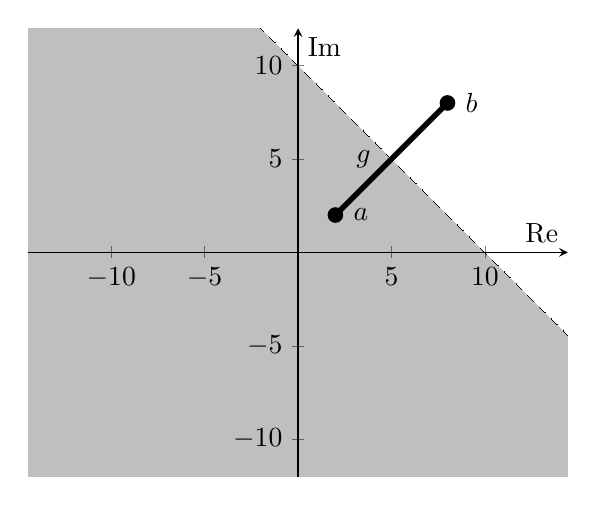
\begin{tikzpicture}
		\begin{axis}[four quad complex, xmin=-12, xmax=12, ymin=-12, ymax=12]
			\draw[line width=0pt,dashed,fill=black,fill opacity=0.25](-20,20)--(-20,-20)--(20,-20)--(20,-10)--(-5,15);
			\draw[color=black] (-1,13) node {$f$};
			\draw[line width=2pt,solid](2,2)--(8,8);
			\draw[color=black] (3.5,5) node {$g$};
			\node[label={0:{$a$}},circle,fill,inner sep=2pt] at (axis cs:2,2) {};
			\node[label={0:{$b$}},circle,fill,inner sep=2pt] at (axis cs:8,8) {};
		\end{axis}
	\end{tikzpicture}
}
\subsection*{Every complex number has exactly 2 roots}
$\forall z = x = iy \in \mathbb{C} \; x, y \in \mathbb{R} \\
\exists w_{1, 2} = u + iv \in \mathbb{C} \; u, v \in \mathbb{R}$
\begin{equation*}
	\resizebox{\columnwidth}{!}{%
		$w = \begin{cases}
			\pm \left[ \left(\frac{x + \sqrt{x^2 + y^2}}{2} \right)^{\frac{1}{2}} + i \left( \frac{-x + \sqrt{x^2 + y^2}}{2} \right)^{\frac{1}{2}} \right] & y > 0 \\
			\pm \left[ \left(\frac{x + \sqrt{x^2 + y^2}}{2} \right)^{\frac{1}{2}} - i \left(\frac{-x + \sqrt{x^2 + y^2}}{2} \right)^{\frac{1}{2}} \right] & y < 0 \\
			\pm \sqrt{x} & y = 0, x > 0 \\
			\pm i \sqrt{x} & y = 0, x < 0
		\end{cases}$
	}
\end{equation*}
\subsection*{Quadratic Formula}
$\forall a, b, c \in \mathbb{C} \; a \neq 0 \; az^2 + bz + c = 0$
\begin{equation*}
	z = \frac{-b + \sqrt{b^2 - 4ac}}{2a}
\end{equation*}
\subsection*{Argument}
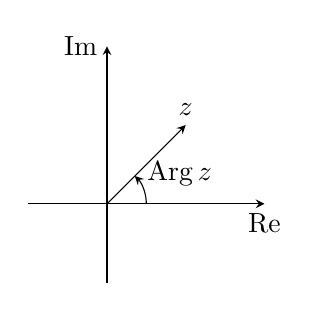
\begin{tikzpicture}
	\tikzset{>=stealth}
	\draw[->] (-1, 0) -- ++(3, 0) coordinate (X) node[below] {$\re$};
	\draw[->] (0, -1) -- ++(0, 3) node[left] {$\im$};
	\coordinate (O) at (0, 0);

	\draw[->] (O) -- (1,1) coordinate (z) node[above] {$z$};
	\path (X) -- (O) -- (z) pic [draw,->,pic text=$\Arg{z}$, angle eccentricity=2.0] {angle=X--O--z};
\end{tikzpicture}
\subsection*{Polar Form}
$\forall z \in \mathbb{C} \; \exists r, \theta \in \mathbb{R} \; \theta \in [0, 2\pi)$ \\
$z = re^{i\theta}$
\subsection*{Polar to Cartesian}
$x = r \cos \theta \quad y = r \sin \theta$
\subsection*{Cartesian to Polar}
$r = \abs{z} \quad \tan \theta = \frac{x}{y}$
\subsection*{Conjugate in Polar Form}
$z = re^{i\theta} \iff \bar{z} = re^{-i\theta}$
\subsection*{Inverse in Polar Form}
$z = re^{i \theta} \land z \neq 0 \\
\implies z^{-1} = \frac{1}{r} e^{-i \theta}$
\subsection*{Product in Polar Form}
\begin{itemize}
	\item $z_1 z_2 = r_1 r_2 e^{i (\theta_1 + \theta_2)}$
	\item $\forall n \in \mathbb{Z} \enspace (re^{in}) = r^n e^{in\theta}$
\end{itemize}
\subsection*{nth Roots of a Complex Number}
$\left\{ r^{\frac{1}{n}} e^{i \left(\frac{\theta + 2 \pi k}{n} \right)} : k = 0, 1, ..., n - 1 \right\}$
\subsection*{nth Roots of Unity}
$\left\{ e^{i \left(\frac{2 \pi k}{n} \right)} : k = 0, 1, ..., n - 1 \right\}$


\end{multicols*}
\end{document}